%ergebnisse.tex
\chapter{Ergebnisse}
\label{sec:Ergebnisse}

Bei einer üblichen Klassifikation im Bereich des maschinellen Lernens mit ausreichend klassifizierten und zudem repräsentativen Trainingsdaten würde man hier nun eine Trainings- und Testphase durchführen. Das bedeutet die Trainingsdaten würden in ein Traningsset und ein Testset aufgeteilt werden. Man würde dann die im Algorithmus verwendeten Parameter anhand des Trainingssets optimieren und dann mit Hilfe des Testsets die allgemeine Performance überprüfen. Wie schon bei der Analyse der Daten festgestellt wurde, ist die Menge der zur Verfügung stehenden Regelsätze weder ausreichend noch repräsentativ für den ganzen Markt. Zur Verfügung stehen die Regelsätze von neun verschiedenen Tankstellen, die alle von einem einzelnen Preishoheitsinhaber gesteuert werden. Es gibt verschiedene Ansätze, wie in diesen Fällen vorgegangen werden kann, um dieses Format trotzdem beibehalten zu können. Es könnte zum Beispiel künstlich ein dem Markt entsprechendes Setup simuliert werden, welches genügend Trainingsdaten erzeugt. Das würde bedeuten, künstlich Tankstellen mit Konkurrenten und Regeln zu erzeugen, authentisches Verhalten zu implementieren und somit einen neuen Datensatz zu erzeugen, anhand dessen vernünftig trainiert werden könnte. Abgesehen davon, dass dafür einige Parameter aus dem originalen Datensatz benötigt würden, um einen authentischen künstlichen Markt zu generieren, würde der Aufwand dafür den Rahmen dieser Arbeit überschreiten. Deshalb werden hier einfach die vorhandenen Daten verwendet.  

\section{Diskussion}
Auch wenn das Ziel nicht war, alle existierenden Regeln zu erkennen, so bieten diese Regeln doch eine gute Grundlage, die generierten Ergebnisse dieses ersten Ansatzes systematisch zu diskutieren. Statt die übliche Optimierung der Parameter  anzustreben soll hier eher genauer dargelegt werden, wie sich verschiedene Einstellungen auf den weiteren Verlauf und die letztlichen Ergebnisse des Programmes auswirken. Dazu wird zunächst ein Testlauf mit den \textit{default} Werten duchgeführt. Dann werden die Ergebnisse und verschiedene andere Faktoren in Vier-Felder-Tafeln dargestellt, um genauer auf die veschiedenen Formen von Fehlklasifikationen eingehen zu können. Zu den besonders auffälligen Werten werden dann Hypothesen aufgestellt, was die Ursachen für diese Ergebnisse sein könnten. Diese Hypothesen werden dann mittels weitere statistiken untermauert werden.

\begin{figure}[!ht]
	\caption{Konkurrenten Entscheidungsgenauigkeit}
	\hspace*{\fill}%
		\subfloat[Default Einstellung]{\label{fig1:DE}
			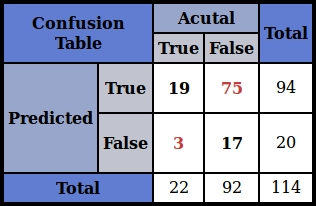
\includegraphics[width=0.3\textwidth]{Bilder/default_comp_overall_acc.jpg}}
		\hfill
		\subfloat[Erhöhte Mindestzahl an potentiellen Konkurrenten]{\label{fig1:EM}
			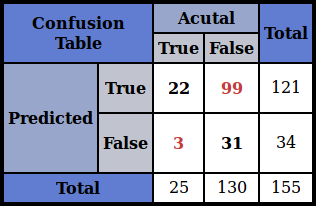
\includegraphics[width=0.3\textwidth]{Bilder/n_val_comp_overall_acc.jpg}}
		\hfill
		\subfloat[Differenz]{\label{fig1:D}
			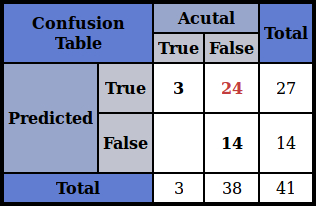
\includegraphics[width=0.3\textwidth]{Bilder/n_val_comp_dif_acc.jpg}}
	\hspace*{\fill}%
	\label{fig:KE}
\end{figure}

Wie in \autoref{fig:KE}\subref{fig1:DE} zu sehen, ist die Zahl der $\beta$-Fehler relativ gering. Es werden also fast alle Konkurrenten erkannt. Bei den nicht erkannten Konkurrenten handelt es sich um Fälle, in denen sich die Anzahl der zu den jeweiligen Regeln gehörenden Reaktionen auf maximal 9 beziehungsweise 2\% beschränkt. Auf die drei Monate verteilt wäre dies nicht einmal eine Reaktion pro Woche. Die Tabelle beinhaltet allerdings nur die untersuchten Tankstellen, also nicht jene, die schon bei der Auswahl der potentiellen Konkurrenten über die Abstandsbestimmung aus dem Raster fallen. Die default Einstellung hat als Abstandsobergrenze 5km, welche sich jeweils verdoppelt, wenn die Mindestanzahl von 5 Konkurrenten nicht erreicht worden ist. Bei diesen Parametern beläuft sich die Anzahl der nicht erfassten Konkurrenten auf drei. Erhöht man die Mindestzahl der Konkurrenten auf 10, so sinkt dieser Wert auf null herab. Allerdings werden bei dieser Einstellung wie in \autoref{fig:KE}\subref{fig1:EM} und \subref{fig1:D} zu sehen insgesamt 41 Tankstellen mehr untersucht, wovon 24 fälschlicherweise auch als Konkurrenten klassifiziert werden. Diese Einstellung würde sich demnach nur lohnen, wenn die Anzahl der $\alpha$-Fehler deutlich reduziert werden kann. Diese hohe Zahl an vermeintlich erkannten Konkurrenten hat vermutlich verschiedene Ursachen. Zunächst sollte natürlich der Konfidenz-Threshold für Konkurrenten betrachtet werden.

\begin{figure}[!ht]
	\center
	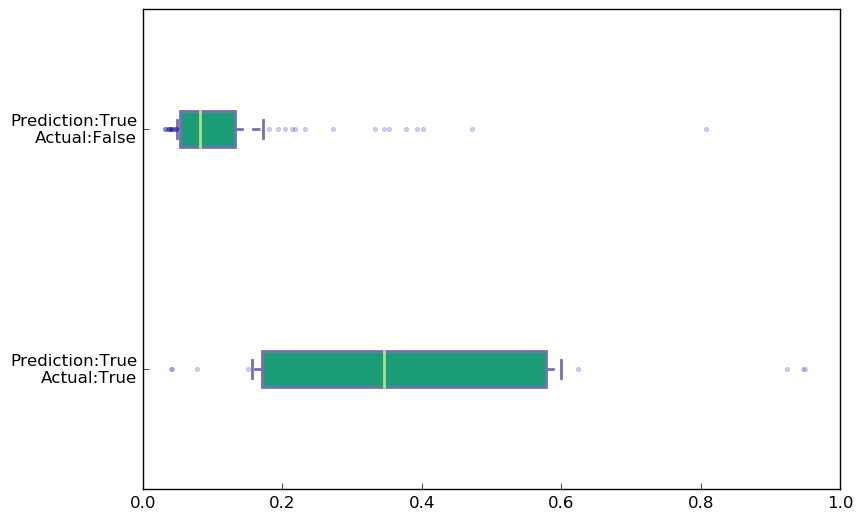
\includegraphics[width=0.6\textwidth]{Bilder/comp_conf_boxplot.png}\\
	\caption{Konkurrenz-Konfidenz-Verteilung}
	\label{fig:KKV}
\end{figure}

\autoref{fig:KKV} zeigt Boxplots der jeweiligen Konfidenzwerte der Konkurrenten und unterscheidet zwischen tatsächlichen Konkurrenten und den fälschlicherweise als Konkurrenten erkannten Tankstellen. Die beiden Fälle, in denen der Algorithmus die Tankstelle nicht als Konkurrenten klassifiziert, sind nicht aufgeführt, da hier alle Konfidenzwerte unter der Untergrenze von 3\% liegen. Würde man den Threshold auf 15\% erhöhen, könnte man in diesem Testszenario die Anzahl der $\alpha$-Fehler um 75\% reduzieren. Allerdings würden dann auch circa 15\% der richtig erkannten Konkurrenten zu $\beta$-Fehlern werden. Die Wahl des Wertes sollte jedoch eher inhaltlich begründet werden, als an den letztendlichen Ergebnissen dieses Tests. Der durchschnittliche Konfidenzwert beträgt bei den tatsächlichen Konkurrenten in etwa 35\% und bei allen anderen ungefähr 10\%. Die 10\% sind demnach so etwas wie eine zufällige Korrelation, die im Mittel zwischen jeder Paarung von Tankstellen existiert. Der Wert fällt allerdings höchstwahrscheinlich ein um einiges höher aus, weil nur benachbarte Tankstellen in diesen Wert eingehen, bei denen zu einem nicht geringen Anteil auch wirklich stark korrelierende Paarungen existieren, die zwar nicht direkt kausal verknüpft sind, sich aber indirekt über dritte Tankstellen parallel verhalten. Anders wären die oberen 10\% der $\alpha$-Fehler in \autoref{fig:KKV} kaum zu erklären.\\
Statistisch gesehen sollte der Threshold dann so gelegt werden, dass signifikante Ausreißer der zufälligen Korrelation zu Konkurrenten erklärt werden. Problematisch bei so einem Ansatz ist, dass die zufällige Korrelation und die kausal bedingte Korrelation so nahe beieinanderliegen, dass sich statistisch vermutlich kein eindeutiger Grenzwert ermitteln lässt. Damit ist gemeint, dass der obere Grenzwert für Ausreißer einer zufälligen Korrelation höher liegt als die Untergrenze für negativ Ausreißer einer kausalen Korrelation. Der Threshold sollte dann in der Schnittmenge liegen, wobei die stärkere Orientierung zu einem der Grenzwerte für Ausreißer eine bestimmte Art von Fehler stärker begünstigt. Der default Wert von 3\% neigt sehr stark dazu, $\beta$-Fehlern zu vermeiden und generiert damit große Mengen an $\alpha$-Fehlern. Erhöht man den Wert auf 10\%, werden 3 $\beta$-Fehler mehr erzeugt während die $\alpha$-Fehler um 42 reduziert werden, was in der Summe der Fehler natürlich eine Steigerung der Performanz bedeuten würde. Alles in allem ist dieser Wert in dieser Form für eine letztendliche Klassifikation nicht besonders gut geeignet.\\
Da dieser Konfidenzwert sehr stark von den erkannten Regeln abhängig ist, können sich auch Veränderungen dort auf die allgemeine Performanz bei den Konkurrenten auswirken. Auch für die Regeln gibt es wieder einen Konfidenzwert, der analysiert werden kann.

\begin{figure}[!ht]
	\center
	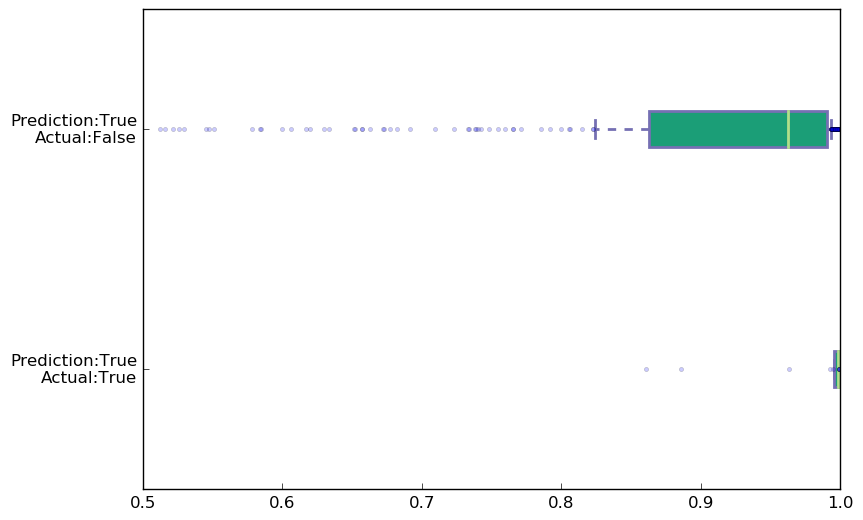
\includegraphics[width=0.6\textwidth]{Bilder/rule_conf_boxplot.png}
	\caption{Regel-Konfidenz-Verteilung}
	\label{fig:RKV}
\end{figure}

Die Idee dieses Wertes war eigentlich, dass nicht die Höhe klassifiziert, ob tatsächlich eine Regel besteht, sondern die Anteile an Reaktionen und ignorierten Preisänderungen, die den Abstand der potentiellen Regel wieder hergestellt beziehungsweise so belassen haben. Hohe Anteile von ignorierten Preisänderungen sollten darauf hindeuten, dass generell keine Konkurrenz besteht und auch nicht weiter nach Regeln gesucht werden muss, während hohe Anteile an Reaktionen eine tatsächliche Regel andeuten sollten. 
Schaut man sich jedoch die Verteilung in \autoref{fig:RKV} an, dann sind die Werte für tatsächliche Regeln eindeutig signifikant höher als bei nicht regelgemäßem Verhalten. Das liegt daran, dass bei nicht regelgemäßem Verhalten die Abstandswerte eine größere Streuung aufweisen. Bei einer Regel sind die Abstandswerte in gewisser Weise nach oben beschränkt, da höhere Abstände sofort wieder auf den der Regel entsprechenden Abstand herabgesetzt werden. Wenn keine Regel vorliegt, verteilen sich die Abstandswerte entsprechend der Höhe der Preisschwankungen auf wenige, aber trotzdem mehrere Werte. Dadurch wird der Eindruck erweckt, es würden mehrere Regeln bestehen. Dieses Verhalten wird auch noch in einigen weiteren Werten sichtbar. Zum Beispiel ist dadurch auch die mittlere Anzahl an Regeln pro Konkurrent bei den tatsächlichen Regeln deutlich niedriger.\\

\begin{figure}[!ht]
	\caption{Regel Treffergenauigkeit}
	\hspace*{\fill}%
		\subfloat[Default Einstellung]{\label{fig1:D}
			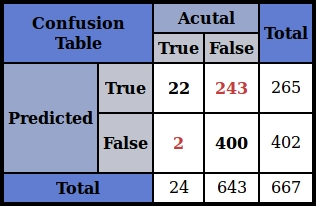
\includegraphics[width=0.3\textwidth]{Bilder/default_rule_overall_acc.jpg}}
		\hfill
		\subfloat[Erhöhte Untergrenze bei dem Konfidenzwert für Regeln]{\label{fig1:ERKU}
			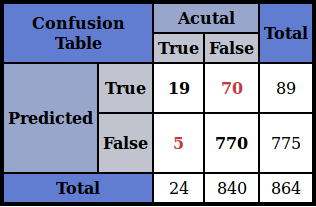
\includegraphics[width=0.3\textwidth]{Bilder/rule_conf_overall_rule_acc.jpg}}
	\hspace*{\fill}%
	\label{fig:RT}

	\bigskip

	\caption{Mittlere Anzahl an Regeln pro Konkurrent}
	\hspace*{\fill}%
		\subfloat[Default Einstellung]{\label{fig1:DMRpK}
			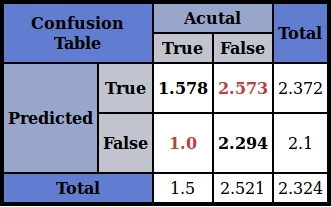
\includegraphics[width=0.3\textwidth]{Bilder/default_avg_num_rules.jpg}}
		\hfill
		\subfloat[Erhöhte Untergrenze bei dem Konfidenzwert für Regeln]{\label{fig1:EMRpK}
			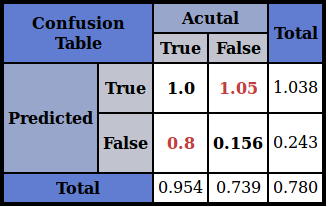
\includegraphics[width=0.3\textwidth]{Bilder/rule_conf_avg_num_rules.jpg}}
	\hspace*{\fill}%
	\label{fig:MRpK}
\end{figure}

\autoref{fig:RT} und \autoref{fig:MRpK} unterstützen diese Erklärung. Hier wurde der Grenzwert für Regeln von dem default Wert 0.5 auf 0.99 erhöht, was sich in der Verteilung der Konfidenzwerte im obigen Boxplot als ein guter Trennwert herausgestellt hat. Die Anzahl der fehlerhaften Regeln nimmt stark ab, weil einfach generell die Anzahl der Regeln abnimmt. Dies hat auch einen positiven Effekt auf die Fehler bei der Klassifikation der Konkurrenten.\\
Andere Möglichkeiten, diesen Umstand auszunutzen, wären demnach, die Anzahl an Regeln per se auf eine einzelne pro Konkurrent zu beschränken oder den Konfidenzwert für Konkurrenten durch die Anzahl an Regeln zu teilen. Alle diese Eingriffe senken die Anzahl der $\alpha$-Fehler bei den Konkurrenten erheblich und verursachen nur eine geringe Anzahl an neuen $\beta$-Fehlern. Das liegt zu großen Teilen aber auch daran, dass in den Testdaten fast nur einzelne Regeln vertreten sind. Bei mehreren Regeln pro Konkurrenten verteilen sich die Abstandswerte auch, hier dann auf die verschiedenen Regeln, und sind somit auch stärker gestreut. Das führt schon bei den wenigen Fällen im Testset mit zwei Regeln für einen Konkurrenten dazu, dass diese nicht mehr erkannt werden. Diese Art von Anpassung würde also nur Sinn machen, wenn man davon ausgehen könnte, dass generell nur eine Regel pro Konkurrent anzunehmen ist.\\
Ein anderer Faktor, der sich bei den $\alpha$-Fehler stark von den tatsächlichen Konkurrenten abhebt, sind die Ausnahmen der Regeln, also die Preisabstände, die oberhalb der Regel innerhalb des relevanten Intervalls auftreten. Dadurch, dass bei mehreren Regeln die jeweiligen Zeitintervalle kleiner sind, bestehen jeweils immer große Intervalle für weitere niedrigere Regeln. In diesen Intervallen, wo prinzipiell Regeln gelten können, welche aber erst von niedrigeren Regeln belegt werden, können dann auch vermehrt höhere Abstände auftreten als bei einer einzelenen Regel über dem ganzen Intervall. Gerade bei Verhalten, welches sich nicht an Regeln orientiert, sind die Werte stark über den ganzen Zeitraum hinweg gestreut und führen so bei kleinen Regelintervallen zu vielen Ausnahmen, die bei jeder weiteren Regel mehr werden. Bei mehreren Regeln und regelkonformem Verhalten sind zwar auch die Intervalle der einzelnen Regeln kleiner, aber die Abstandswerte beschränken sich weitgehend, das heißt bis auf einzelne Ausreißer, auf das für die Regel gültige Intervall. Deshalb bleibt hier auch ein Unterschied erhalten, wenn man den Mindestkonfidenzwert für Regeln erhöht und so generell weniger Regeln klassifiert werden.\\

\begin{figure}[!ht]
	\center
	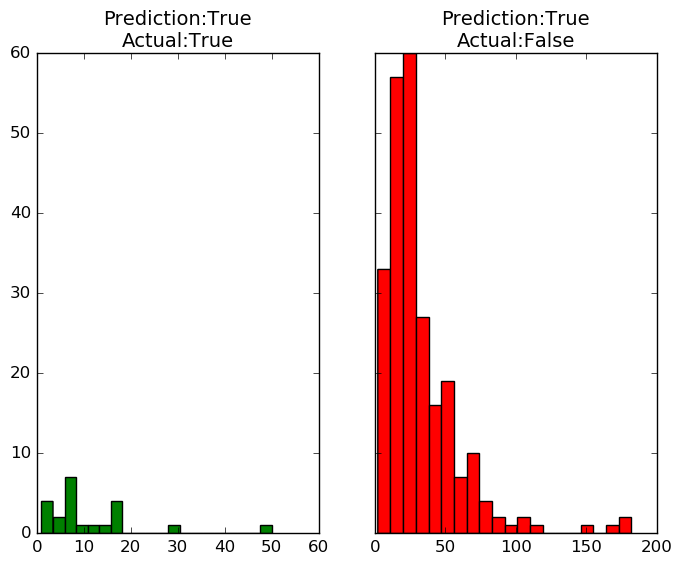
\includegraphics[width=0.6\textwidth]{Bilder/exception_hist.png}\\
	\caption{Regel-Ausnahmen-Verteilung}
	\label{fig:RAV}
\end{figure}

\autoref{fig:RAV} zeigt den starken Unterschied bei den Ausnahmen zwischen tatsächlichen und vermeintlichen Regeln. Die Ausnahmen in diesen Konfidenzwert mit einzuberechnen sollte die Klassifikation hier also deutlich verbessern.\\
Vor dem Hintergrund wird auch ersichtlich, dass es wichtig ist, sich die Intervalle der Regeln genauer anzuschauen. In Testdaten gelten die Regeln immer an allen Tagen, weshalb bei den Tagesintervallen keine neuen Erkenntnisse zu erwarten sind. Die Güte der Klassifikation an sich ist auch nicht besonders aussagekräftig. Es wurden zwar für die Statistik nur die Regeln ausgewählt, wo letzlich auch eine Konkurrenz vermutet wurde. Allerdings ist es bei der Höhe der $\alpha$-Fehler bei den Konkurrenten und den Regeln dann auch nicht verwunderlich, dass bei den Stunden hier erhebliche Mengen an Fehlern bestehen. Interessant sind Werte, die helfen, Regeln aufgrund von unplausiblen Intervallen zurückzuweisen, um eben die Klassifikation von Regeln zu verbessern. Hier sind vor allem zwei Faktoren interessant.
\begin{figure}[!ht]
	\caption{Generelle Stunden Statistiken}
	\hspace*{\fill}%
		\subfloat[Stunden Treffgenauigkeit]{\label{fig1:ST}
			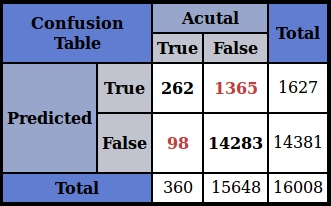
\includegraphics[width=0.3\textwidth]{Bilder/default_hour_overall_acc.jpg}}
		\hfill
		\subfloat[Mittlere Anzahl an Stunden pro Regel]{\label{fig1:MSpR}
			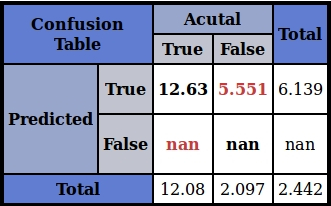
\includegraphics[width=0.3\textwidth]{Bilder/default_avg_num_hours.jpg}}
	\hspace*{\fill}%
	\label{fig:GSS}

	\bigskip

	\caption{Angepasste Stunden Statistiken}
	\hspace*{\fill}%
		\subfloat[Anteil an Regeln mit geänderten Stunden]{\label{fig1:ARgS}
			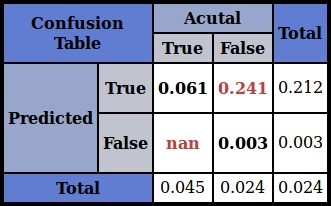
\includegraphics[width=0.3\textwidth]{Bilder/default_avg_hours_changed.jpg}}
		\hfill
		\subfloat[Mittlere Anzahl an geänderten Stunden pro Regel]{\label{fig1:MgSpR}
			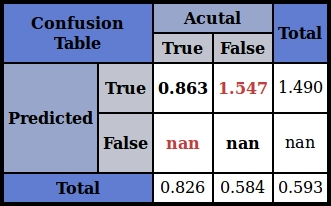
\includegraphics[width=0.3\textwidth]{Bilder/default_avg_num_hours_changed.jpg}}
	\hspace*{\fill}%
	\label{fig:GS}
\end{figure}
\autoref{fig:GSS} zeigt zum einen, dass sich die tatsächlichen Regeln von den fälschlicherweise erkannten erheblich in der Anzahl an Stunden pro Intervall unterscheiden. Zum anderen wurde bei den Stunden gerade wegen den teilweise unregelmäßigen Verteilungen auch bei tatsächlichen Regeln eine Art Smoothing verwendet, was einzelne Ausreißer in der Klassifikation an die Werte der Umgebung angepasst hat. Das sollte in erster Linie dazu führen, dass einzelne Regeln begünstigt werden sollten und nicht allzu kleine Intervalle entstehen. Zudem besteht bei der default Einstellung eine Mindestgröße für Regeln nach der sich der Filter für das Smoothing richtet. Die Werte für die tatsächlichen Regeln lassen vermuten, dass dies in diesem Fall auch hilfreich ist. Die nan Werte kommen zustande, weil bei zurückgewiesenen Regeln nicht das Zeitintervall überprüft wird, was dazu führt, dass in diesen Felder eventuell durch null geteilt werden würde.\\
Wie in der \autoref{fig:GS} zu sehen ist, wurden in wenigen Fällen einige negative Ausreißer mit ins Intervall aufgenommen, was zu einer Durchschnittslänge von 12.63 geführt hat. Dabei sollte wieder berücksichtigt werden, dass kleinere Intervalle auch kaum in den Testdaten vorkommen. Die Statistik zeigt aber auch, dass das Smoothing bei fehlerhaft erkannten Regeln viel häufiger und gleichzeitig auch absolut mehr Stunden in das Intervall mit aufgenommen hat. Trotzdem wurden dadurch im Durchschnitt mit 5.5 Stunden nur sehr kurze Intervalle erkannt. Bei 1.5 angepassten Stunden pro falscher Regel sind also mehr als ein Viertel der Stunden wegen ihrer Umgebung trotzdem in das Intervall aufgenommen worden. Das Verfahren ist also in dieser Form noch nicht besonders hilfreich. Es sollte ein anderes Vorgehen entworfen werden, was größere Intervalle noch stärker unterstützt und bei starker Streuung auch die Möglichkeit besitzt, eine Regel zurückzuweisen. Das würde zwar wahrscheinlich auch wieder die existierenden Konkurrenten mit mehreren Regeln mit jeweils nur wenigen Stunden benachteiligen, allerdings sollte eine Aufteilung in verschiedene Regeln an einem Tag auch inhaltlich begründet sein. Man sollte annehmen können, dass bei kurzen Intervallen ein besonderes Augenmerk auf diese Konkurrenz gelegt wurde und dass in diesem Intervall auch einige Änderungen stattfinden, die der gesonderten Anpassung bedürfen. Es sollte dort also von einer geringeren Streuung ausgegangen werden können. Ab einem gewissen Punkt, also kurze Intervalle mit starker Streuung, wäre es auch schlicht nicht mehr möglich und inhaltlich sinnvoll begründbar, diese als gesonderte Regeln zu identifizieren.
\begin{figure}[!ht]
	\caption{Erhöhte Mindestanzahl an Stunden pro Regel}
	\hspace*{\fill}%
		\subfloat[Anteil an Regeln mit geänderten Stunden]{\label{fig1:EARgS}
			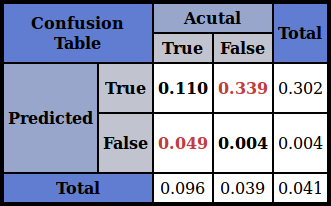
\includegraphics[width=0.3\textwidth]{Bilder/hour_min_avg_hours_changed.jpg}}
		\hfill
		\subfloat[Mittlere Anzahl an geänderten Stunden pro Regel]{\label{fig1:EMgSpR}
			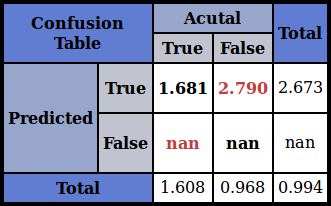
\includegraphics[width=0.3\textwidth]{Bilder/hour_min_avg_num_hours_changed.jpg}}
	\hspace*{\fill}%
	\label{fig:EMSpR}
\end{figure}
\autoref{fig:EMSpR} zeigt noch einmal, dass eine einfache Erhöhung der Mindeststundenanzahl noch keine Abhilfe schafft. Die Mindestanzahl wurde hier von 3 auf 5 erhöht. Bei den letztendlichen Klassifikationen wurde so keinerlei Verbesserungen erzeugt. Die Änderung hat lediglich bewirkt, dass noch häufiger und noch mehr Stunden lediglich aufgrund ihrer Umgebung in die Intervalle aufgenommen wurden.\\
